\documentclass[12pt]{article}
\usepackage{../../../../format}
\lhead{A Level Physics - Turning Points}

%File specific preamble
\usepackage{textcomp}


\begin{document}
\begin{center}
\underline{\huge Newton\textquotesingle s Corpuscular Theory of light}
\end{center}
Definition - Light is made up of tiny particles called corpuscles that always travel in a straight line
\section{Reflection and refraction}
Newton believed this theory was true as it can explain both reflection and refraction\\
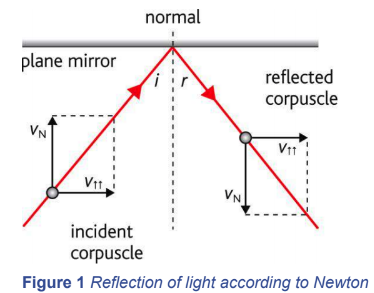
\includegraphics[width=6cm]{reflection.png}
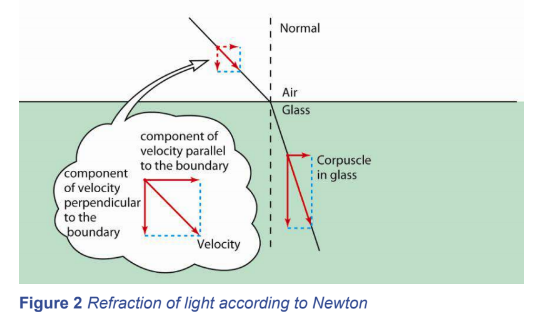
\includegraphics[width=6cm]{refraction.png}\\
\\
\textbf{Reflection} - There is a short range repulsive force.These corpuscles have perfectly elastic collisions, meaning that the speed before is the speed after. The horizontal velocity doesn't change, the vertical velocity is inverted. Therefore angle of incidence equals angle of reflection.\\
\\
\textbf{Refraction} - There is a short range attractive force. Newton said the corpuscles were attracted into the material, causing them to travel faster, causing the component of the velocity perpendicular to the boundary to increase, causing angle with the normal to reduce. Newton was wrong.
\section{Rival theories}
Christiaan Huygens proposed the wave front theory, which is the theory we have been taught to describe refraction and diffraction. This described light travelling slower in a more dense material.\\
\\
Why Huygens' theory was rejected:
\begin{itemize}
\item It was not possible to measure the speed of light at that scale at that time, meaning neither theory could be proved correct or incorrect.
\item Newton had a better reputation
\item The wave theory only considered longitudinal waves so couldn't explain polarisation.
\end{itemize}

\end{document}